\documentclass{standalone}

\usepackage{pgf}
\usepackage{tikz}
\usetikzlibrary{arrows,automata,positioning}
\usepackage[latin1]{inputenc}

\tikzset{every loop/.style={min distance=18mm}}
\tikzset{node distance=2.5cm,
	every state/.style={
		semithick,
		fill=gray!10
	},
	initial text={
		\begin{tabular}{cl}
			1 & $\wedge$ \\
			\hline
			\ & sendBase =\\
			\ & nextSequence =\\
			  & 1
		\end{tabular}},
	double distance=2pt,
	every edge/.style={
		draw,
		->,>=stealth',
		auto,
		semithick
	}
}
\begin{document}
	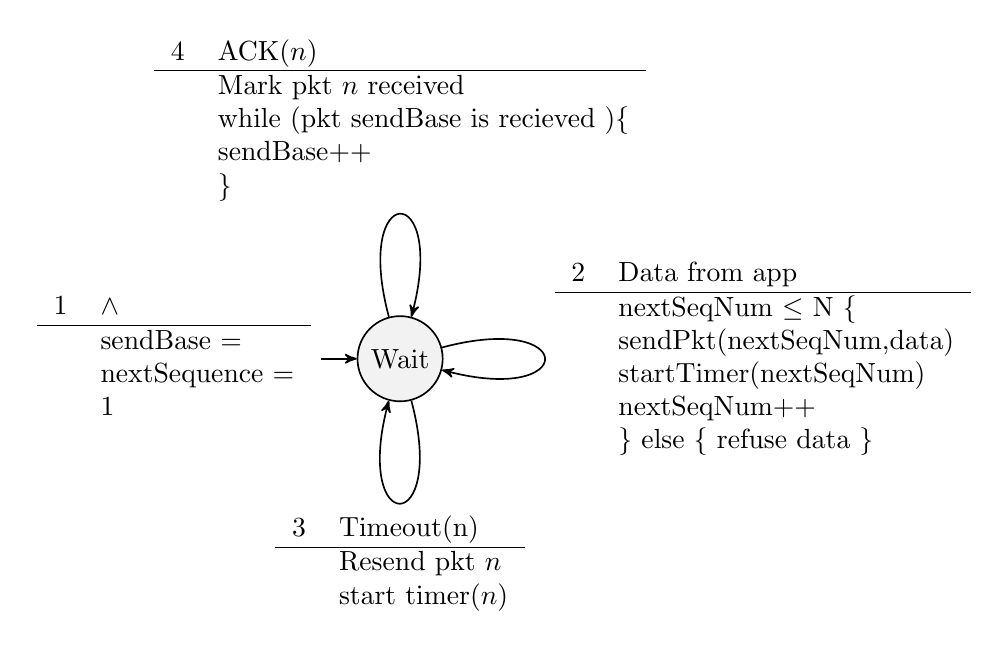
\begin{tikzpicture}
		\node[initial, state] (c) {Wait};
		\draw (c) edge[loop right] node{
			\begin{tabular}{cl}
				2 & Data from app\\
				\hline
				  & nextSeqNum $\le$ N \{\\
				  & sendPkt(nextSeqNum,data)\\
				  & startTimer(nextSeqNum)\\
				  & nextSeqNum++ \\
				  & \} else \{ refuse data \}
			\end{tabular}
		} (c)
		(c) edge[loop below] node{
			\begin{tabular}{cl}
				3 & Timeout(n)\\
				\hline
				  & Resend pkt $n$\\
				  & start timer($n$)
			\end{tabular}
		} (c)
		(c) edge[loop above] node{
			\begin{tabular}{cl}
				4 & ACK($n$)\\
				\hline
				  & Mark pkt $n$ received\\
				  & while (pkt sendBase is recieved )\{\\
				  & sendBase++\\
				  & \}
			\end{tabular}
		} (c);
	\end{tikzpicture}
\end{document}
